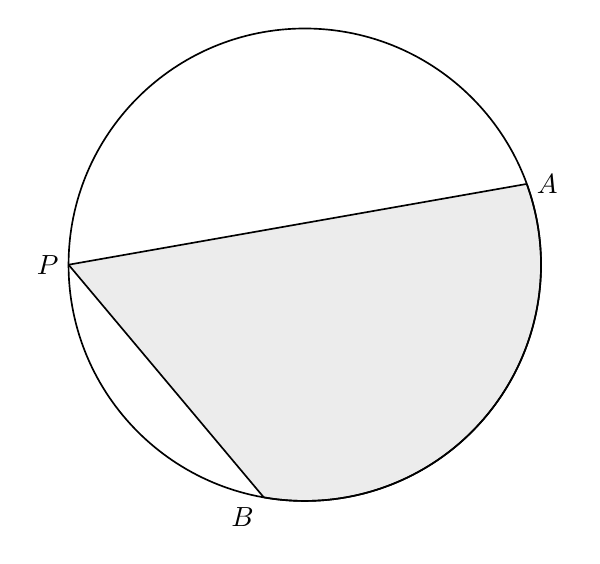
\begin{tikzpicture}[x=1cm,y=1cm,line width=.6pt,font=\normalsize]
\coordinate (O) at (0,0);
\coordinate (P) at (-3,0);
\coordinate (A) at (2.819,1.026);
\coordinate (B) at (-0.521,-2.954);
\fill[fill=gray!15,draw=none] (P)--(A) arc[start angle=20,end angle=-100,radius=3cm] -- cycle;
\draw (O) circle[radius=3cm];
\draw (P)--(A);
\draw (P)--(B);
\draw (A) arc[start angle=20,end angle=-100,radius=3cm];
\node[left] at (P) {$P$};
\node[right] at (A) {$A$};
\node[below left] at (B) {$B$};
\end{tikzpicture}
